\documentclass{beamer}
\usetheme{Madrid}
\usecolortheme{default}

% ==================== PACKAGES ====================
\usepackage{graphicx}
\usepackage{booktabs}
\usepackage{amsmath}
\usepackage{amsfonts}
\usepackage{tabularx}
\usepackage{hyperref}
\usepackage{colortbl}
\usepackage{xcolor}

% ==================== COLOR DEFINITIONS ====================
\definecolor{themeblue}{RGB}{30, 70, 140}
\definecolor{lightgray}{RGB}{245, 245, 245}
\definecolor{advgreen}{RGB}{220, 245, 220}
\definecolor{limred}{RGB}{255, 225, 225}

% ==================== METADATA ====================
\title[Generative Agents in ABM]{\textbf{GENERATIVE AGENTS IN AGENT-BASED MODELING}}
\subtitle{Overview, Validation and Emerging Challenges}

\author{
\textbf{Submitted by:} \\ Aravind A Kamath (CEC23CS041) \\[0.5cm]
\textbf{Under the Guidance of:} \\ Mrs. JAYASREE K \\ Assistant Professor
}
\institute{
\\[0.05cm]
Department of Computer Science and Engineering \\ College of Engineering, Cherthala
}

\date[\today]{}

\begin{document}

% ==================== SLIDE 1: TITLE SLIDE ====================
\begin{frame}
  \titlepage
\end{frame}

% ==================== SLIDE 2: OUTLINE ====================
\begin{frame}{Presentation Outline}
\tableofcontents
\end{frame}

% ==================== SECTION 1 ====================
\section{Introduction and Theoretical Foundations}

% ==================== SLIDE 3: BACKGROUND OF ABM ====================
\begin{frame}{Background: Agent-Based Modeling (ABM)}
\textbf{Definition and Scope:}
\begin{itemize}
    \item Computational simulation of autonomous entities (agents) interacting locally.
    \item Primary objective: Observe emergent macroscopic patterns from micro-level decisions.
\end{itemize}

\medskip
\textbf{Traditional Agent Mechanics:}
\begin{itemize}
    \item Built on rigid mathematical equations, heuristics or 'if-then' rules.
    \item Assumes strict economic rationality (\textit{homo economicus}).
\end{itemize}

\medskip
\textbf{Core Limitations:}
\begin{itemize}
    \item Fails to capture human bounded rationality, bias and emotional states.
    \item Cannot model natural language dialogue or open-ended reasoning.
\end{itemize}
\end{frame}

% ==================== SLIDE 4: GENERATIVE SOCIAL SCIENCE ====================
\begin{frame}{The Concept of 'Generative' in Social Science}
\textbf{Historical Terminology (Epstein, 1999):}
\begin{itemize}
    \item Core principle: \textit{"If you didn't grow it, you didn't explain it."}
    \item In classical ABM, 'generative' meant growing macro structures from local micro rules without central coordination.
\end{itemize}

\medskip
\textbf{Foundational Classical Models:}
\begin{itemize}
    \item \textbf{Schelling's Segregation (1971):} Mild individual neighbor preferences generate extreme macroscopic segregation.
    \item \textbf{Reynolds' Boids (1987):} Lifelike flocking emerges from three local rules (Separation, Alignment, Cohesion).
\end{itemize}

\medskip
\textbf{The Modern Terminological Shift:}
\begin{itemize}
    \item Classical generative models did \textbf{not} utilize generative artificial intelligence.
    \item Modern GABMs explicitly leverage Large Language Models (LLMs) to synthesize autonomous cognitive behaviors.
\end{itemize}
\end{frame}

% ==================== SLIDE 5: CASE STUDY COMPARISON (TABLE I) ====================
\begin{frame}{Traditional ABM vs. Generative ABM: Urban Traffic Flow}
\scriptsize
\begin{table}[h]
\centering
\caption{\scriptsize{Comparison of the same simulation scenario under ABM and GABM (Table I of base paper)}}
\begin{tabularx}{\textwidth}{p{2.2cm}X p{5.3cm}}
\toprule
\textbf{Dimension} & \textbf{Traditional ABM} & \textbf{Generative ABM (GABM)} \\
\midrule
\textbf{Scenario} & Traffic flow in a city with cars managed by signals and road closures. & Traffic flow incorporating human social norms, emotions and communication. \\
\midrule
\textbf{Objective} & Optimizes physical throughput, predicts congestion bottlenecks, visually graphs flow. & Uncovers how social norms, personal risk, stress and individual decisions shape mobility patterns. \\
\midrule
\textbf{Outcomes \& Generalization} & Produces context-specific engineering outputs for urban planners; findings cannot generalize into broader social theories. & Generates theoretical insights into social behavior-infrastructure interplay; generalizable across domains. \\
\midrule
\textbf{Decision Basis} & Purely rational shortest-path algorithms (Dijkstra/A*), ignoring subjective mental states. & Context-sensitive reasoning accounting for fear, comfort, scenic preference and social influence. \\
\bottomrule
\end{tabularx}
\end{table}
\end{frame}

% ==================== SECTION 2 ====================
\section{Evolution of Agents in ABM}

% ==================== SLIDE 6: EVOLUTIONARY ALGORITHMS ====================
\begin{frame}{Evolution of Agents: Evolutionary Algorithms (EAs)}
\textbf{Darwinian Principles in ABM:}
\begin{itemize}
    \item Introduces adaptation through selection, mutation and crossover.
    \item Genetic Algorithms (GAs) and Evolution Strategies optimize agent parameters via fitness functions.
\end{itemize}

\medskip
\textbf{Cultural Algorithms and Belief Spaces:}
\begin{itemize}
    \item Maintains an explicit shared 'belief space' (population-level knowledge repository).
    \item Extracts collective experiences to guide individual agent evolution.
\end{itemize}

\medskip
\textbf{Key Limitations of EA Approaches:}
\begin{itemize}
    \item High computational cost from iterative multi-generation evaluations.
    \item Risk of premature convergence to suboptimal local equilibria.
    \item High sensitivity to hyperparameter tuning (mutation rates, selection pressure).
\end{itemize}
\end{frame}

% ==================== SLIDE 7: REINFORCEMENT LEARNING ====================
\begin{frame}{Evolution of Agents: Reinforcement Learning (RL)}
\textbf{Trial-and-Error Policy Optimization:}
\begin{itemize}
    \item Agents optimize actions to maximize cumulative reward signals.
    \item Applications: Pedestrian dynamics, evacuation routes and financial markets.
\end{itemize}

\medskip
\textbf{Key Challenges in Social Simulations:}
\begin{itemize}
    \item \textbf{Stochasticity \& Suboptimality:} Early exploration causes erratic behaviors; easily trapped in local optima.
    \item \textbf{Brittle Generalization:} Policies struggle when deployed in novel, data-scarce social environments.
    \item \textbf{Lack of Language:} Optimizes numerical state tensors without support for semantic dialogue, negotiation or persuasion.
\end{itemize}
\end{frame}

% ==================== SLIDE 8: AI IN ABM DEVELOPMENT (FIGURE 1) ====================
\begin{frame}{AI Integration in ABM Development}
\begin{itemize}
    \item Machine Learning integrates into ABM across two primary areas: \textbf{Structural Specification} and \textbf{Output Analysis}.
\end{itemize}

% ==================== FIGURE 1 PLACEMENT GUIDE ====================
% Figure 1 from Section III-A (Page 4 of base paper).
% Caption in Paper: AI can be used in two distinct areas of ABM development: Structural specification and output analysis. Over them, generative AI can contribute to population synthesis, decision making through interactions and scenario generation.
% Visual Elements: Tree breakdown showing Structural Specification vs Output Analysis and Generative AI spanning across both.
% Filename to use: fig1_ai_in_abm.png
\begin{figure}[h]
    \centering
    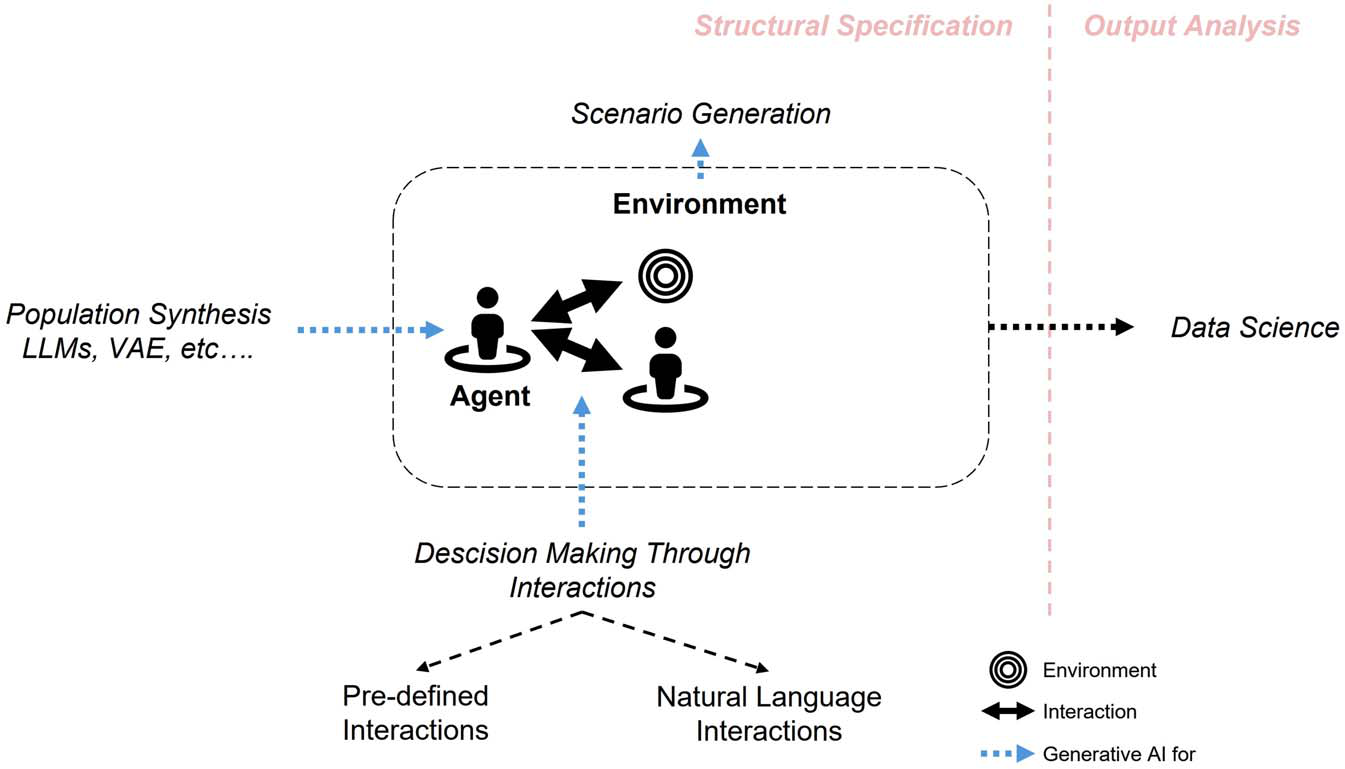
\includegraphics[width=0.80\textwidth]{fig1_ai_in_abm.png}
    \caption{Key roles of Generative AI in ABM development (Source: Base Paper, Section III-A)}
\end{figure}

\begin{itemize}
    \item \textbf{Population Synthesis:} Generates synthetic demographic agents; behaviors remain static ex-ante.
    \item \textbf{Decision Making via Interactions:} LLMs dynamically generate decisions from evolving interaction history (true GAs).
    \item \textbf{Scenario Generation:} Generative models construct and characterize dynamic synthetic environments.
\end{itemize}
\end{frame}

% ==================== SECTION 3 ====================
\section{Architecture and Mechanics of Generative Agents}

% ==================== SLIDE 9: DEFINITION AND FEEDBACK LOOP ====================
\begin{frame}{Defining Generative Agents (GAs)}
\begin{itemize}
    \item \textbf{Formal Definition:}
    \begin{itemize}
        \item A Generative Agent (GA) is an autonomous computational entity powered by a Large Language Model, capable of displaying human-like behavior, reasoning contextually and interacting via natural language.
    \end{itemize}
    \medskip
    \item \textbf{The LLM Feedback Loop Concept:}
    \begin{itemize}
        \item Environmental feedback loop: The simulation environment and agents continuously exchange feedback regarding states and actions with the underlying LLM.
        \item \textbf{Mechanical Model:} Rule-based physical substrate defined by developers (coordinates, physics, obstacle collision, time progression).
        \item \textbf{Cognitive Layer:} Large Language Model interprets the sensory perception, queries its internal knowledge and memories and generates believable behavioral responses.
    \end{itemize}
    \medskip
    \item \textbf{Key Breakthrough:}
    \begin{itemize}
        \item Behavioral rules emerge organically from pre-trained world knowledge rather than being rigidly pre-programmed by researchers.
    \end{itemize}
\end{itemize}
\end{frame}

% ==================== SLIDE 10: INFERENTIAL VS CONVERSATIONAL (FIGURE 2A, 2B) ====================
\begin{frame}{GA Decision Architectures: Inferential vs. Conversational}
% ==================== FIGURE 2(A, B) PLACEMENT GUIDE ====================
% Figure 2(a) and 2(b) from Section IV (Page 5 of base paper).
% Caption in Paper: LLM-based feedback loop and status of GAs. (a) Inferential GA feedback loop where LLM produces discrete action; (b) Conversational GA feedback loop where LLM decides based on natural language interactions which directly update status.
% Filename to use: fig2_ga_feedback_loop_status.png
\begin{figure}[h]
    \centering
    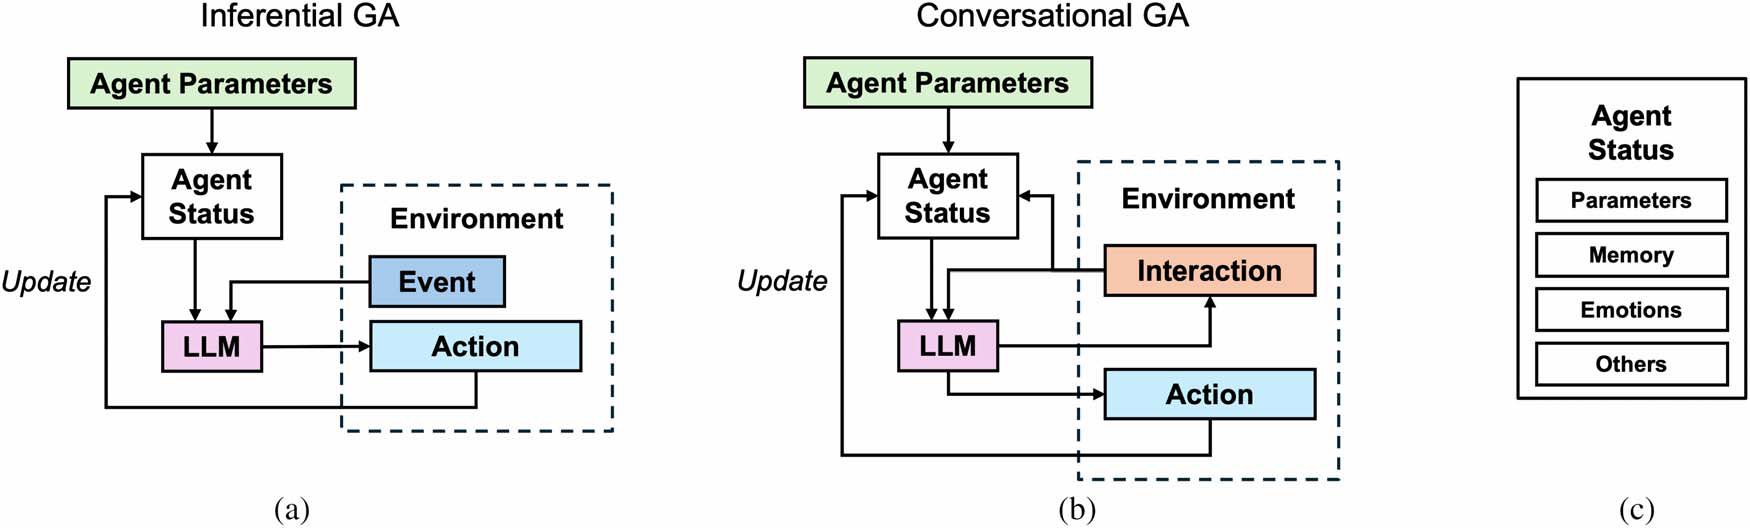
\includegraphics[width=0.85\textwidth]{fig2_ga_feedback_loop_status.png}
    \caption{\scriptsize{LLM-based feedback loop architectures for Generative Agents (Source: Base Paper, Section IV)}}
\end{figure}
\begin{itemize}
    \item \textbf{Inferential GAs [Fig. 2(a)]:}
    \begin{itemize}
        \item LLM serves purely as a centralized decision engine.
        \item Inputs: Current Agent Status + Environmental Event $\rightarrow$ Output: Discrete Action.
    \end{itemize}
    \item \textbf{Conversational GAs [Fig. 2(b)]:}
    \begin{itemize}
        \item Agents engage in open-ended natural language exchanges with peers.
        \item Dialogues directly alter internal beliefs, relationships and emotional statuses.
    \end{itemize}
\end{itemize}
\end{frame}

% ==================== SLIDE 11: PARAMETERS AND AGENT STATUS ====================
\begin{frame}{Internal State Representation: Parameters vs. Dynamic Status}
\textbf{Agent Parameters (Static Baseline):}
\begin{itemize}
    \item \textbf{Demographics:} Age, gender, income tier, occupation, education.
    \item \textbf{Psychological Profile:} Big Five personality traits (OCEAN).
    \item \textbf{Social Network:} Baseline relationships, family ties and roles.
\end{itemize}

\bigskip
\textbf{Dynamic Agent Status (Runtime Representation):}
\begin{itemize}
    \item \textbf{State Representation:} Captures agent state during simulation runtime.
    \item \textbf{Decoupled Architecture:} Separates internal state from LLM decision logic.
    \item \textbf{Affective Tracking:} Records dynamic sentiment, emotional shifts and interaction history.
\end{itemize}
\end{frame}

% ==================== SLIDE 12: MEMORY STREAM AND RETRIEVAL ====================
\begin{frame}{Core Cognitive Components: Memory Stream \& Retrieval}
\begin{itemize}
    \item \textbf{Memory Stream (Park et al., 2023):}
    \begin{itemize}
        \item A comprehensive chronological database recording all sensory observations, natural language dialogues and internal thoughts.
        \item Overcomes LLM finite context window limits by externalizing long-term experience storage.
    \end{itemize}
    \medskip
    \item \textbf{Contextual Multi-Factor Retrieval Function:}
    \begin{itemize}
        \item Whenever an agent decides or speaks, it queries its memory stream using a weighted linear combination of three normalized scores:
    \end{itemize}
\end{itemize}
\begin{equation*}
    \text{Score} = \alpha \cdot \text{Recency} + \beta \cdot \text{Importance} + \gamma \cdot \text{Relevance}
\end{equation*}
\begin{itemize}
    \item \textbf{Recency:} Exponential decay function prioritizing recent events over distant memories.
    \item \textbf{Importance:} Integer score assigned by LLM separating trivial routines (e.g., brushing teeth) from pivotal events (e.g., job offer).
    \item \textbf{Relevance:} Cosine similarity between embedding vector of current context and memory statement embedding.
\end{itemize}
\end{frame}

% ==================== SLIDE 13: REFLECTION HIERARCHY AND PLANNING ====================
\begin{frame}{Core Cognitive Components: Reflection \& Dynamic Planning}
\begin{itemize}
    \item \textbf{Reflection Hierarchy (Knowledge Synthesis):}
    \begin{itemize}
        \item Raw sensory observations are insufficient for high-level social intelligence.
        \item The reflection module periodically triggers when accumulated importance scores cross a threshold.
        \item Queries the 100 most recent memories, synthesizes patterns and generates higher-level abstract thoughts.
        \item Forms an evolving directed tree: Base observations (leaf nodes) $\rightarrow$ Abstract beliefs and values (higher-level nodes).
    \end{itemize}
    \medskip
    \item \textbf{Planning and Reactive Execution Loop:}
    \begin{itemize}
        \item \textbf{Top-Down Plan Decomposition:} Agents formulate realistic broad daily agendas, recursively decomposing them into hourly schedules, then minute-by-minute action sequences.
        \item \textbf{Dynamic Reactive Re-planning:} When an unexpected event or conversation occurs, the agent pauses its schedule, re-evaluates through the LLM and updates its plan adaptively.
    \end{itemize}
\end{itemize}
\end{frame}

% ==================== SECTION 4 ====================
\section{Notable Implementations and Frameworks}

% ==================== SLIDE 14: SMALLVILLE ====================
\begin{frame}{Notable Implementations: The Smallville Sandbox}
\begin{itemize}
    \item \textbf{Experimental Sandbox (Park et al., 2023):}
    \begin{itemize}
        \item 2D sprite environment (resembling \textit{The Sims}) populated by 25 autonomous generative agents.
        \item Agents initialized with simple text seed descriptions (name, occupation, basic relationships).
    \end{itemize}
    \medskip
    \item \textbf{Emergent Macroscopic Phenomena:}
    \begin{itemize}
        \item \textbf{Information Diffusion:} When one agent announced a desire to host a Valentine's Day party, the news organically diffused across the town over two simulation days through peer-to-peer dialogues.
        \item \textbf{Autonomous Coordination:} Agents independently decorated the venue, invited friends and showed up at the party at the specified hour without hardcoded triggers.
        \item \textbf{Emergent Social Ties:} Agents formed new friendships and political opinions regarding town mayoral elections.
    \end{itemize}
    \medskip
    \item \textbf{Ablation Findings:}
    \begin{itemize}
        \item Removing either Memory, Reflection or Planning severely degraded agent believability and long-term behavioral coherence.
    \end{itemize}
\end{itemize}
\end{frame}

% ==================== SLIDE 15: CONCORDIA AND SOTOPIA ====================
\begin{frame}{General-Purpose Simulation Frameworks}
\begin{itemize}
    \item \textbf{Concordia (Google DeepMind / Vezhnevets et al., 2023):}
    \begin{itemize}
        \item General-purpose simulation framework for language-mediated interactions in grounded digital, physical or social spaces.
        \item Introduces a centralized \textbf{'Game Master'} agent: Grounds language actions into physical reality, enforcing physical constraints, resource budgets and institutional rules.
        \item Bridges unconstrained LLM text generation with structured environmental state transitions.
    \end{itemize}
    \medskip
    \item \textbf{SOTOPIA (Zhou et al., 2024):}
    \begin{itemize}
        \item Open-ended interactive environment designed to evaluate social intelligence in language agents.
        \item Simulates complex, goal-driven interpersonal scenarios involving cooperation, competition, deception and negotiation.
        \item Features cross-agent profiles and provides quantitative benchmarks for multi-agent social dialogues.
    \end{itemize}
\end{itemize}
\end{frame}

% ==================== SLIDE 16: NORMS (CRSEC) AND NETWORKS (S3) ====================
\begin{frame}{Social Norm Emergence and Online Networks}
\begin{itemize}
    \item \textbf{CRSEC Architecture for Social Norm Emergence (2024):}
    \begin{itemize}
        \item Four-stage cognitive pipeline modeling how social norms naturally emerge and get enforced in GA societies:
        \begin{enumerate}
            \item \textbf{Creation \& Representation:} Formalizes novel behavioral rules from observed social friction.
            \item \textbf{Spreading:} Disseminates normative expectations through peer conversations.
            \item \textbf{Evaluation:} Agents assess conformity and compute social sanction penalties.
            \item \textbf{Compliance:} Internalizes rules into future planning routines.
        \end{enumerate}
        \item Successfully validated with 10 GAs in Smallville (e.g., establishing indoor smoking bans).
    \end{itemize}
    \medskip
    \item \textbf{S3: Social-Network Simulation System (Gao et al., 2023):}
    \begin{itemize}
        \item Models digital information propagation, emotional contagion and echo chamber polarization across virtual online platforms.
        \item Empirically replicates real-world retweet cascades and opinion divergence.
    \end{itemize}
\end{itemize}
\end{frame}

% ==================== SECTION 5 ====================
\section{Validation Methodologies for ABM and GABM}

% ==================== SLIDE 17: THE VALIDATION DILEMMA ====================
\begin{frame}{The Fundamental Validation Dilemma}
\begin{itemize}
    \item \textbf{Why Validation is Essential:}
    \begin{itemize}
        \item Critical for establishing trust, credibility and ensuring simulation findings reflect real-world social processes rather than computational artifacts.
    \end{itemize}
    \medskip
    \item \textbf{The Core Epistemological Hurdle:}
    \begin{itemize}
        \item Traditional ABM agents are transparent white-box models: Explicit rules can be mathematically inspected.
        \item Generative Agents are non-deterministic, probabilistic black boxes: Multiple runs with identical inputs produce divergent outputs.
        \item Internal reasoning paths cannot be uniformly traced back to closed-form equations.
    \end{itemize}
    \medskip
    \item \textbf{Hierarchy of Evidence (inspired by Evidence-Based Medicine):}
    \begin{itemize}
        \item \textbf{Highest Rigor:} Ecological validity and controlled experimental trials.
        \item \textbf{Intermediate:} Observational field data matching.
        \item \textbf{Lowest Rigor:} Theoretical plausibility and expert consistency.
    \end{itemize}
\end{itemize}
\end{frame}

% ==================== SLIDE 18: FOUNDATIONAL & ADVANCED ABM VALIDATION ====================
\begin{frame}{Traditional ABM Validation Methods}
\small
\begin{itemize}
    \item \textbf{Foundational Validation Methods (Base Paper Section V-A):}
    \begin{itemize}
        \item \textbf{Data Analytics:} Statistical cleaning, feature correlation and input/output distribution verification.
        \item \textbf{Docking (Model Alignment):} Comparing simulation outputs against established baseline models under identical parameters.
        \item \textbf{Empirical Validation:} Matching simulated macroscopic outputs against observed historical datasets.
        \item \textbf{Sampling:} Sensitivity testing across parameter spaces to evaluate model robustness.
    \end{itemize}
    \medskip
    \item \textbf{Advanced Validation Methods:}
    \begin{itemize}
        \item \textbf{Bootstrapping:} Resampling simulation runs to build empirical confidence intervals without assuming normal distributions.
        \item \textbf{Causal Analysis:} Evaluating intervention effects to distinguish genuine causality from spurious correlations.
        \item \textbf{Inverse Generative Social Science (IGSS):} Using genetic programming to backward-engineer agent rule structures that produce target macro-patterns.
        \item \textbf{Spatial Analytics:} Validating topological and geographic distribution patterns.
    \end{itemize}
\end{itemize}
\end{frame}

% ==================== SLIDE 19: FACE VALIDATION ====================
\begin{frame}{Face Validation: Qualitative and Human-Centric}
\begin{itemize}
    \item \textbf{Definition of Face Validation:}
    \begin{itemize}
        \item Assessment of whether model operational mechanics and outputs appear realistic, believable and plausible to human domain experts.
    \end{itemize}
    \medskip
    \item \textbf{Microface Validation:}
    \begin{itemize}
        \item Evaluates individual agent behaviors at the micro-level.
        \item Verifies that personal choices, emotional transitions and natural language statements are logically coherent and believable over time.
    \end{itemize}
    \medskip
    \item \textbf{Macroface Validation:}
    \begin{itemize}
        \item Examines aggregate, system-level simulation patterns (e.g., crowd evacuation flows, spatial segregation, traffic bottlenecks).
        \item Assesses whether collective emergent behaviors match intuitive real-world expectations.
    \end{itemize}
    \medskip
    \item \textbf{Immersive Assessment:}
    \begin{itemize}
        \item Allows human experts to enter the virtual environment directly (via interactive UI or VR) to interview agents and evaluate responses in real time.
    \end{itemize}
\end{itemize}
\end{frame}

% ==================== SLIDE 20: GABM VALIDATION WORKFLOWS ====================
\begin{frame}{GABM Validation Workflows: The Integrated Architecture}
\centering
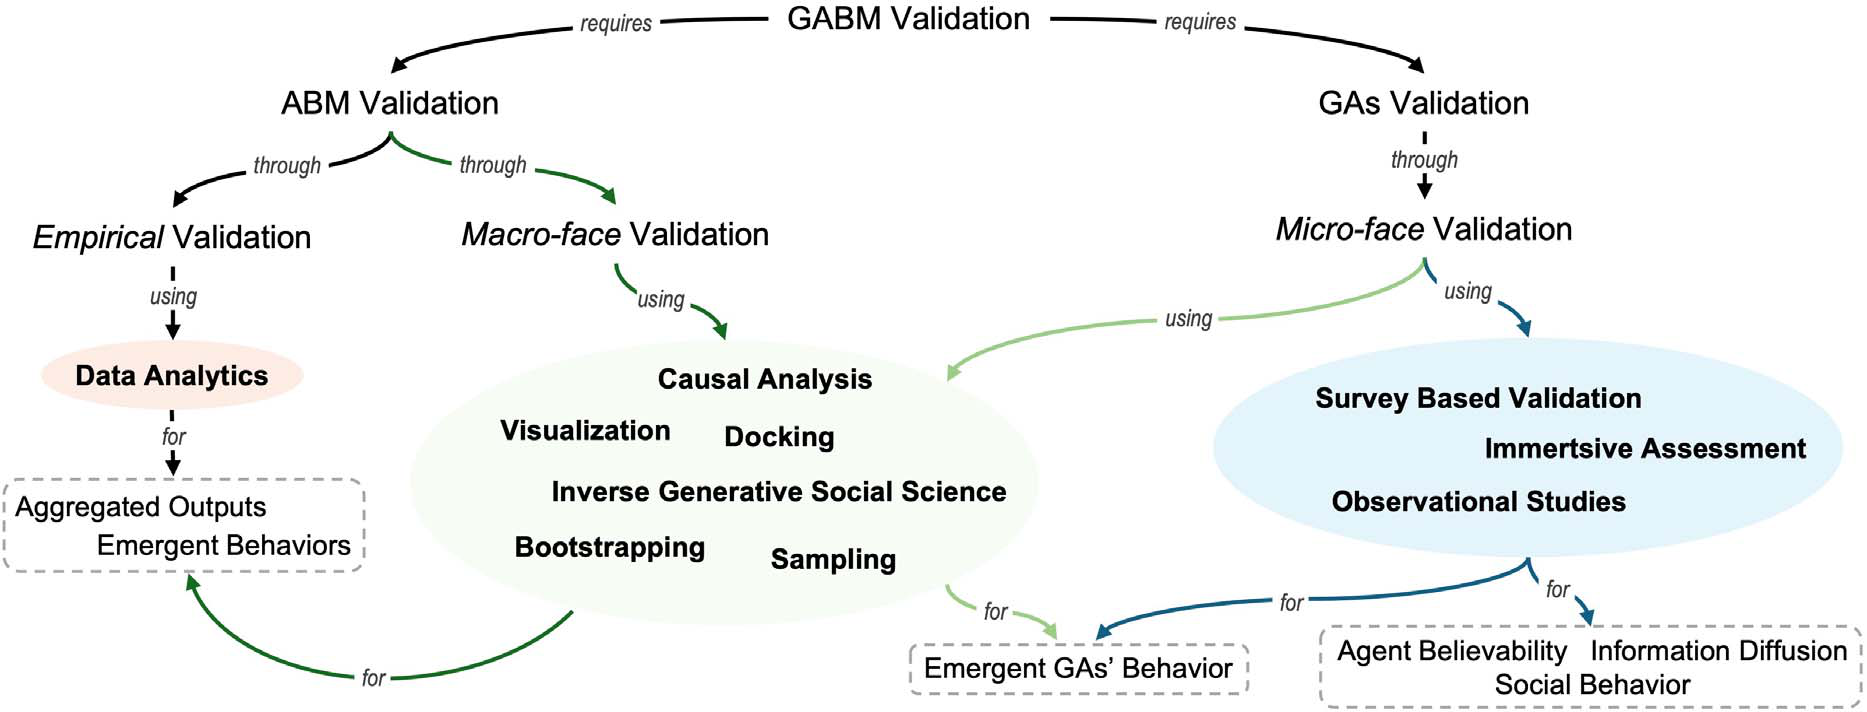
\includegraphics[width=0.9\textwidth,height=0.46\textheight,keepaspectratio]{fig3_gabm_validation_workflows.png}

\vspace{0.15cm}
\begin{itemize}\small
    \item \textbf{Empirical Pathway:} Data analytics and docking for quantitative macro-matching.
    \item \textbf{Macroface Pathway:} Spatial and causal analysis for collective emergent patterns.
    \item \textbf{Microface Pathway:} Interviews, believability scoring and dialogue audits.
\end{itemize}
\end{frame}

% ==================== SLIDE 21: CONTROLLED EVALUATION & SOTOPIA-EVAL ====================
\begin{frame}{Validating Existing GAs: Empirical Implementations}
\begin{itemize}
    \item \textbf{Smallville Controlled Evaluation (Park et al., 2023):}
    \begin{itemize}
        \item Human evaluators interviewed agents across five core cognitive categories:
        \begin{enumerate}
            \item Self-Knowledge \quad 2. Memory \quad 3. Plans \quad 4. Reactions \quad 5. Reflections
        \end{enumerate}
        \item Evaluated 100 human judges across 5 ablation conditions to measure believability.
    \end{itemize}
    \medskip
    \item \textbf{SOTOPIA-EVAL Benchmark (Zhou et al., 2024):}
    \begin{itemize}
        \item Quantitative evaluation framework measuring social intelligence across 7 dimensions:
        \begin{itemize}
            \item \textbf{Goal Completion:} Objective task attainment.
            \item \textbf{Believability:} Human-like plausibility of speech.
            \item \textbf{Knowledge Gained:} Contextual information absorbed.
            \item \textbf{Secret Keeping:} Information containment and privacy adherence.
            \item \textbf{Relationship Dynamics:} Trust and rapport trajectory.
            \item \textbf{Social Norm Adherence:} Respect for cultural conventions.
            \item \textbf{Financial Benefits:} Economic resource preservation.
        \end{itemize}
    \end{itemize}
\end{itemize}
\end{frame}

% ==================== SLIDE 22: AUTOMATED AND HYBRID EVALUATION ====================
\begin{frame}{Automated Validation: LLM-as-a-Judge \& Algorithmic Fidelity}
\textbf{LLM-as-a-Judge (Automated Evaluation):}
\begin{itemize}
    \item Uses independent LLMs to interview agents and grade dialogues at scale.
    \item \textbf{Strengths:} Evaluates objective goals and quantitative metrics effectively.
    \item \textbf{Limitations:} Struggles with nuanced social conventions, sarcasm and deception.
    \item \textbf{Takeaway:} Demands hybrid pipelines combining AI grading with human oversight.
\end{itemize}

\medskip
\textbf{Fidelity and Generalization Principles:}
\begin{itemize}
    \item \textbf{Algorithmic Fidelity:} Measures how accurately conditioned personas mirror genuine human demographic attitudes.
    \item \textbf{Similarity Principle:} Rigorous validation on sample scenarios builds statistical confidence across related unobserved spaces.
\end{itemize}
\end{frame}

% ==================== SECTION 6 ====================
\section{Comparative Analysis: Traditional ABM vs. GABM}

% ==================== SLIDE 23: COMPARISON: RESOURCES AND DESIGN ====================
\begin{frame}{Comparison: Resources and Agent Design (Table III)}
\centering
\scriptsize
\begin{tabularx}{\textwidth}{p{3.2cm}X X X X}
\toprule
\textbf{Dimension} & \textbf{Rule-Based} & \textbf{EA-Based} & \textbf{RL-Based} & \textbf{GABM} \\
\midrule
\multicolumn{5}{l}{\textbf{Resources:}} \\
Computational Efficiency & \cellcolor{advgreen}High & \cellcolor{limred}Moderate & \cellcolor{limred}Low & \cellcolor{limred}Low \\
Scalability (Millions) & \cellcolor{advgreen}High & \cellcolor{advgreen}Moderate & \cellcolor{limred}Low & \cellcolor{limred}Very Low \\
Data Independence & \cellcolor{limred}Data-Dependent & \cellcolor{limred}Data-Dependent & \cellcolor{limred}Data-Dependent & \cellcolor{advgreen}Data-Less \\
\midrule
\multicolumn{5}{l}{\textbf{Agent Design:}} \\
Control over Agents & \cellcolor{advgreen}Strict / Direct & \cellcolor{advgreen}High & \cellcolor{limred}Moderate & \cellcolor{limred}Low \\
Learning During Sim & \cellcolor{limred}Static & \cellcolor{advgreen}Evolutionary & \cellcolor{advgreen}Continuous & \cellcolor{limred}Unpractical \\
Real-Time Optimization & \cellcolor{advgreen}Not Needed & \cellcolor{limred}Required & \cellcolor{limred}Required & \cellcolor{advgreen}Not Needed \\
Hyperparameter Tuning & \cellcolor{advgreen}Minimal & \cellcolor{limred}Heavy & \cellcolor{limred}Heavy & \cellcolor{advgreen}Prompt-Based \\
Fast Prototyping & \cellcolor{limred}Labor-Intensive & \cellcolor{limred}Moderate & \cellcolor{limred}Slow & \cellcolor{advgreen}Very Rapid \\
\bottomrule
\end{tabularx}

\vspace{0.15cm}
\raggedright\tiny
\textbf{Key Takeaways (Base Paper, Table III):}
\begin{itemize}\tiny
    \item Green denotes advantage; Red denotes limitation.
    \item GABMs enable data-less simulations and rapid prototyping, but trade off computational scalability.
\end{itemize}
\end{frame}

% ==================== SLIDE 24: COMPARISON: BEHAVIOR AND VALIDATION ====================
\begin{frame}{Comparison: Agent Behavior and Validation (Table III)}
\centering
\scriptsize
\begin{tabularx}{\textwidth}{p{3.2cm}X X X X}
\toprule
\textbf{Dimension} & \textbf{Rule-Based} & \textbf{EA-Based} & \textbf{RL-Based} & \textbf{GABM} \\
\midrule
\multicolumn{5}{l}{\textbf{Agent Behavior:}} \\
Determinism & \cellcolor{advgreen}Deterministic & \cellcolor{limred}Stochastic & \cellcolor{limred}Stochastic & \cellcolor{limred}Stochastic \\
Reliable Decision-Making & \cellcolor{advgreen}Guaranteed & \cellcolor{limred}Suboptimal Risk & \cellcolor{limred}Early Instability & \cellcolor{limred}Hallucination Risk \\
Cognitive Functions & \cellcolor{limred}None & \cellcolor{limred}None & \cellcolor{limred}Primitive & \cellcolor{advgreen}Advanced \\
Natural Language Inter & \cellcolor{limred}None & \cellcolor{limred}None & \cellcolor{limred}None & \cellcolor{advgreen}Human-like \\
Nuanced Mental Models & \cellcolor{limred}None & \cellcolor{limred}None & \cellcolor{limred}None & \cellcolor{advgreen}Beliefs/Emotions \\
\midrule
\multicolumn{5}{l}{\textbf{Validation:}} \\
Decision Transparency & \cellcolor{advgreen}White-Box & \cellcolor{advgreen}Traceable & \cellcolor{limred}Black-Box & \cellcolor{limred}Black-Box \\
Validation Efficiency & \cellcolor{advgreen}High (Automated) & \cellcolor{advgreen}Moderate & \cellcolor{advgreen}Quantitative & \cellcolor{limred}Resource-Intensive \\
Direct Human Interaction & \cellcolor{limred}No & \cellcolor{limred}No & \cellcolor{limred}No & \cellcolor{advgreen}Direct Interview \\
\bottomrule
\end{tabularx}

\vspace{0.15cm}
\raggedright\tiny
\textbf{Key Takeaways (Base Paper, Table III):}
\begin{itemize}\tiny
    \item GABMs uniquely provide rich cognitive modeling and direct natural language human interview validation.
    \item Traditional ABMs guarantee strict determinism and transparent, white-box decision logic.
\end{itemize}
\end{frame}

% ==================== SECTION 7 ====================
\section{Emerging Challenges in GABMs}

% ==================== SLIDE 25: HALLUCINATIONS ====================
\begin{frame}{Challenge 1: Large Language Model Hallucinations}
\begin{itemize}
    \item \textbf{Definition and Taxonomy (Base Paper Section VIII-A):}
    \begin{itemize}
        \item Generation of ungrounded, fabricated or contextually inconsistent text.
        \item \textbf{Factuality Hallucinations:} Contradicting verified real-world facts (e.g., claiming Edison invented the telephone) or fabricating unverifiable information.
        \item \textbf{Faithfulness Hallucinations:} Diverging from assigned persona parameters, contradicting prior conversation history or exhibiting internal self-contradiction.
    \end{itemize}
    \medskip
    \item \textbf{Mitigation Mechanisms Identified in Paper:}
    \begin{itemize}
        \item \textbf{Data Stage:} Pre-filtering training datasets and Retrieval-Augmented Generation (RAG) to ground prompts in external knowledge stores.
        \item \textbf{Training Stage:} Sensitive neuron dropout and Reinforcement Learning from Human Feedback (RLHF).
        \item \textbf{Inference Stage:} Constrained decoding grammars and multi-agent peer verification loops (agents cross-check claims before acting).
    \end{itemize}
\end{itemize}
\end{frame}

% ==================== SLIDE 26: COMPUTATIONAL COMPLEXITY ====================
\begin{frame}{Challenge 2: Computational Bottlenecks and Scaling}
\begin{itemize}
    \item \textbf{Transformer Attention Overhead:}
    \begin{itemize}
        \item Quadratic inference scaling: $\text{Complexity} = \mathcal{O}(n^2 \cdot d)$ ($n$ = tokens, $d$ = dimension).
        \item High generation latency at each agent decision step.
    \end{itemize}
    \medskip
    \item \textbf{Multi-Agent Scaling Explosion:}
    \begin{itemize}
        \item Pairwise communication across $N$ agents scales as $\mathcal{O}(N^2)$.
        \item Massive LLM API call volume and GPU memory demands.
    \end{itemize}
    \medskip
    \item \textbf{Memory Retrieval Latency:}
    \begin{itemize}
        \item Vector similarity searches scale between $\mathcal{O}(\log N)$ and $\mathcal{O}(N)$.
    \end{itemize}
    \medskip
    \item \textbf{The Scalability Gap:}
    \begin{itemize}
        \item Traditional ABMs simulate $10^5$ to $10^6$ entities on single workstations.
        \item Pure GABMs remain computationally bounded to dozens or hundreds of agents.
    \end{itemize}
\end{itemize}
\end{frame}

% ==================== SECTION 8 ====================
\section{Discussion and Proposed Hybrid Architecture}

% ==================== SLIDE 27: CITIES AS A NATURAL TESTBED ====================
\begin{frame}{Discussion: Cities as a Natural Testbed for GABMs}
\begin{itemize}
    \item \textbf{Why Urban Communities are Ideal:}
    \begin{itemize}
        \item Cities are structured yet dynamic social systems shaped by infrastructure, public policy, community norms and diverse human interactions.
        \item LLMs inherently encapsulate human civic values, social etiquette and cultural behavioral archetypes from pre-training text corpora.
    \end{itemize}
    \medskip
    \item \textbf{Qualitative Experience Mapping (Urban Planning):}
    \begin{itemize}
        \item Traditional urban models focus strictly on functional metrics: Commute times, road capacities, throughput.
        \item GABMs enable the modeling of subjective feelings: Visualizing emotional highs and lows (comfort, fear, anxiety, pleasure) across urban neighborhoods.
        \item Informs human-centric public policy: Designing parks, pedestrian pathways and public housing that actively support emotional well-being.
    \end{itemize}
\end{itemize}
\end{frame}

% ==================== SLIDE 28: COMBINED HYBRID ARCHITECTURE ====================
\begin{frame}{The Proposed Solution: Combined Hybrid ABM-GABM}
\begin{itemize}
    \item \textbf{Core Philosophy: Complementary Synergy, Not Replacement:}
    \begin{itemize}
        \item Base paper argues that ABM and GABM should not be viewed as mutually exclusive competitors.
        \item The optimal paradigm combines the high scalability and speed of rule-based ABMs with the cognitive depth of GABMs.
    \end{itemize}
    \medskip
    \item \textbf{Layered Division of Operational Labor:}
    \begin{itemize}
        \item \textbf{Low-Level Layer (Traditional ABM Algorithms):}
        \begin{itemize}
            \item Handles deterministic, high-frequency physical mechanics: Collision detection, obstacle avoidance, kinematic equations, basic routing ($\mathcal{O}(1)$ or $\mathcal{O}(N)$ speed).
        \end{itemize}
        \item \textbf{High-Level Layer (Generative Agents via LLMs):}
        \begin{itemize}
            \item Invoked only during critical decision bifurcations: Ethical dilemmas, emotional panic responses, negotiations and social cooperation.
        \end{itemize}
    \end{itemize}
\end{itemize}
\end{frame}

% ==================== SLIDE 29: HYBRID CASE STUDY AND VALIDATION ====================
\begin{frame}{Case Study: Building Evacuation \& Hybrid Validation}
\begin{itemize}
    \item \textbf{Illustrative Example: Emergency Building Fire Evacuation:}
    \begin{itemize}
        \item \textbf{Low-Level Rule Engine:} Guides agents around physical corridors, doorways and obstacles via deterministic pathfinding algorithms.
        \item \textbf{High-Level Generative Agent:} When an agent encounters a trapped, injured stranger, it queries the LLM:
        \begin{itemize}
            \item Weighs personal panic vs. social empathy, moral responsibility and perceived fire threat.
            \item Makes a context-sensitive human choice: Risk its life to assist or flee immediately.
        \end{itemize}
    \end{itemize}
    \medskip
    \item \textbf{Hybrid Validation in Practice:}
    \begin{itemize}
        \item \textbf{Macro-Validation:} Quantitative sensor data analytics to ensure aggregate evacuation bottleneck densities match real-world building drill statistics.
        \item \textbf{Micro-Validation:} Interactive natural language interviews to verify individual agent survival reasoning and altruistic decision plausibility.
    \end{itemize}
\end{itemize}
\end{frame}

% ==================== SECTION 9 ====================
\section{Conclusion and References}

% ==================== SLIDE 30: CONCLUSION ====================
\begin{frame}{Conclusion and Key Insights}
\begin{itemize}
    \item \textbf{Summary of Contributions from Base Paper:}
    \begin{enumerate}
        \item \textbf{Paradigm Shift:} GABMs redefine computational social science by replacing rigid rationality assumptions with cognitively plausible, conversational agents.
        \item \textbf{Systematic Terminology:} Clarified the distinction between classical 'generative' social science (Epstein) and modern generative AI simulations.
        \item \textbf{Validation Blueprint:} Synthesized foundational statistical validation with human-centric face validation, interview mechanisms and LLM-as-a-Judge benchmarking.
        \item \textbf{The Path Forward:} The future of scalable social modeling lies in hybrid ABM-GABM architectures, unifying mechanical efficiency with psychological depth.
    \end{enumerate}
    \medskip
    \item \textbf{Open Research Horizons:}
    \begin{itemize}
        \item Developing standardized open-domain social benchmarks.
        \item Formulating algorithmic safeguards against hallucination and bias contamination.
        \item Efficient hybrid execution frameworks for urban-scale policy testing.
    \end{itemize}
\end{itemize}
\end{frame}

% ==================== SLIDE 31: REFERENCES ====================
\begin{frame}{References (Base Paper and Foundational Literature)}
\fontsize{7.5pt}{8.5pt}\selectfont
\setlength{\itemsep}{1pt}
\begin{thebibliography}{6}
\bibitem{adornetto2025}
C.~Adornetto, A.~Mora, K.~Hu, L.~I.~Garcia, P.~Atchade-Adelomou, G.~Greco, et al.,
\newblock ``Generative agents in agent-based modeling: Overview, validation and emerging challenges,''
\newblock \textit{IEEE Trans. Artif. Intell.}, vol.~6, no.~12, pp.~3165--3184, Dec. 2025.

\bibitem{park2023}
J.~S.~Park, J.~C.~O'Brien, C.~J.~Cai, M.~R.~Morris, P.~Liang and M.~S.~Bernstein,
\newblock ``Generative agents: Interactive simulacra of human behavior,''
\newblock in \textit{Proc. 36th ACM UIST}, 2023, pp.~1--22.

\bibitem{zhou2024}
X.~Zhou et al.,
\newblock ``SOTOPIA: Interactive evaluation for social intelligence in language agents,''
\newblock in \textit{Proc. 12th ICLR}, 2024.

\bibitem{vezhnevets2023}
A.~S.~Vezhnevets et al.,
\newblock ``Generative agent-based modeling with actions grounded in physical, social or digital space using Concordia,''
\newblock \textit{arXiv:2312.03664}, 2023.

\bibitem{epstein1999}
J.~M.~Epstein,
\newblock ``Agent-based computational models and generative social science,''
\newblock \textit{Complexity}, vol.~4, no.~5, pp.~41--60, 1999.

\bibitem{horton2023}
J.~J.~Horton,
\newblock ``Large language models as simulated economic agents: What can we learn from Homo Silicus?''
\newblock \textit{NBER Working Paper}, Tech. Rep. w31122, 2023.
\end{thebibliography}
\end{frame}

% ==================== SLIDE 32: THANK YOU ====================
\begin{frame}
\centering
\vspace{1.5cm}
\Huge{\textbf{\textcolor{themeblue}{Thank You!}}} \\[0.8cm]
\Large{\textbf{Questions \& Discussion}} \\[1.0cm]
\end{frame}

\end{document}